In diesem Abschnitt soll der durch den in \ref{3-1-1_arbeitsbericht_tassenerkennung} beschriebene Arbeitsprozess entstandene Algorithmus für die automatische Kamerakalibrierung beschrieben werden. Das Ziel des Algorithmus ist es, die Kanten der rechten Seite des Tisches (siehe \ref{fig:kamerakalibrierung-tischkanten}) zu detektieren um eine Transformation vom Kamera- ins Weltkoordinatensystem zu berechnen. Der Ablauf des Algorithmus ist in \ref{fig:algorithmus-kamerakalibrierung} dargestellt. Zunächst wird der Canny-Algorithmus zur Kantendetektion auf das Bild angewendet. Anschließend werden die Kantenpixel mittels Hough-Transformation in einen dualen Parameterraum transformiert, in dem durch die Suche nach Häufungen zu den Tischkanten korrespondierende Geraden extrahiert werden können. Anschließend werden die zu den Tischkanten gehörigen Punkte aus der Punktwolke extrahiert. Aus diesen Punkten werden mittels des RANSAC Algorithmus Geraden aus der Punktwolke segmentiert. Zudem wird auch die Tischplatte mittels des RANSAC Algorithmus aus der Punktwolke segmentiert. Die gefundenen Geraden werden unter Zuhilfename des ermittelten Normlenvektors der Tischplatte so rotiert, dass sie parallel zur x-y-Ebene verlaufen. Die zum Roboterarm zeigende Kante wird als y-Achse verwendet, während die zweite Kante als x-Achse fungiert. Die z-Achse ergibt sich aus dem Normalenvektor. Den Ursprung des Weltkoordinatensystems bildet das Zentrum des Tisches, welches aus x- und y-Achse sowie den bekannten Maßen des Tisches berechnet werden kann. Eine Darstellung der automatisch detektierten Achsen ist in Abbildung \ref{fig:camera_calibration} dargestellt. Sollte das Ergebnis nicht zufriedenstellend sein, so kann die Kalibrierung auch manuell über eine simple Benutzeroberfläche nachkorrigiert werden wie in Abbildung \ref{fig:calibration_collection} dargestellt.
\begin{figure}
    \centering
    \begin{minipage}{0.45\textwidth}
        \centering
        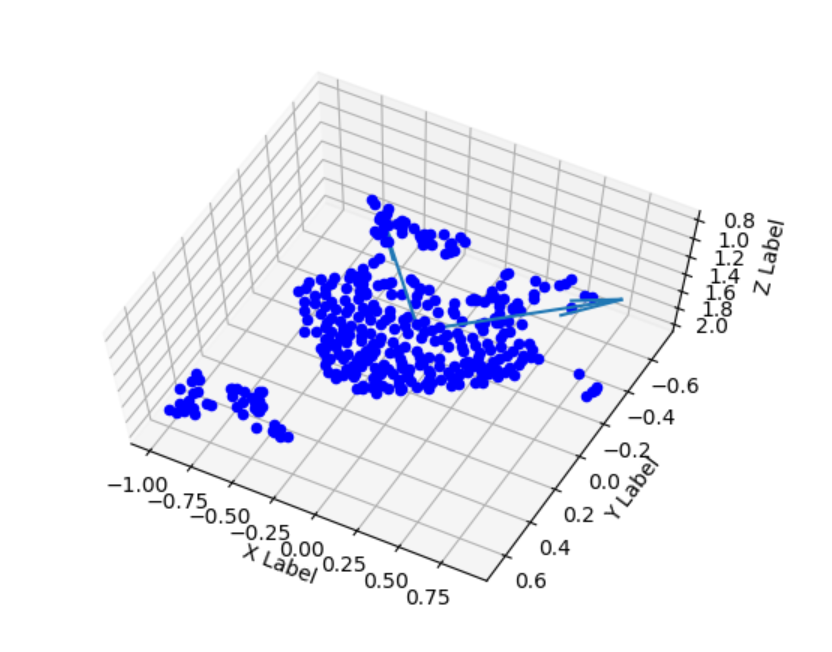
\includegraphics[width=0.9\textwidth]{images/table_automatic_axis_center_estimation.png}
        \caption{Ergebnis der automatischen Kamerakalibrierung \label{fig:camera_calibration}}
    \end{minipage}\hfill
    \begin{minipage}{0.45\textwidth}
        \centering
        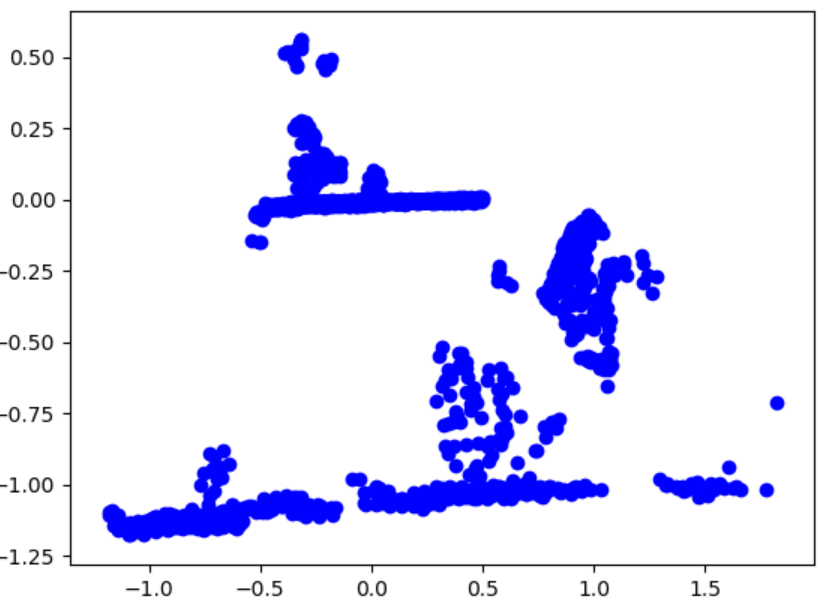
\includegraphics[width=0.9\textwidth]{images/table_manual_calibration.png}
        \caption{Oberfläche bei der manuellen Kalibrierung \label{fig:calibration_collection}}
    \end{minipage}
\end{figure}